\begin{frame}
    \frametitle{Optimization Tool's Design Goals}
    \begin{minipage}[c]{0.45\textwidth}
    \begin{itemize}
        %\item ROLLO (Reactor evOLutionary aLgorithm Optimizer) is a Python package 
        %that applies evolutionary algorithms to optimize nuclear reactor design
        \item The tool couples an evolutionary algorithm driver, Distributed 
        Evolutionary Algorithms in Python (DEAP), with 
        nuclear software, such as neutron transport OpenMC and thermal-hydraulics 
        Moltres codes
        \item Design Goals: effective, flexible, open-source, parallel,
        reproducible
    \end{itemize}
    \end{minipage}\hfill
    \begin{minipage}[c]{0.52\textwidth}
        \centering
        \begin{figure}
            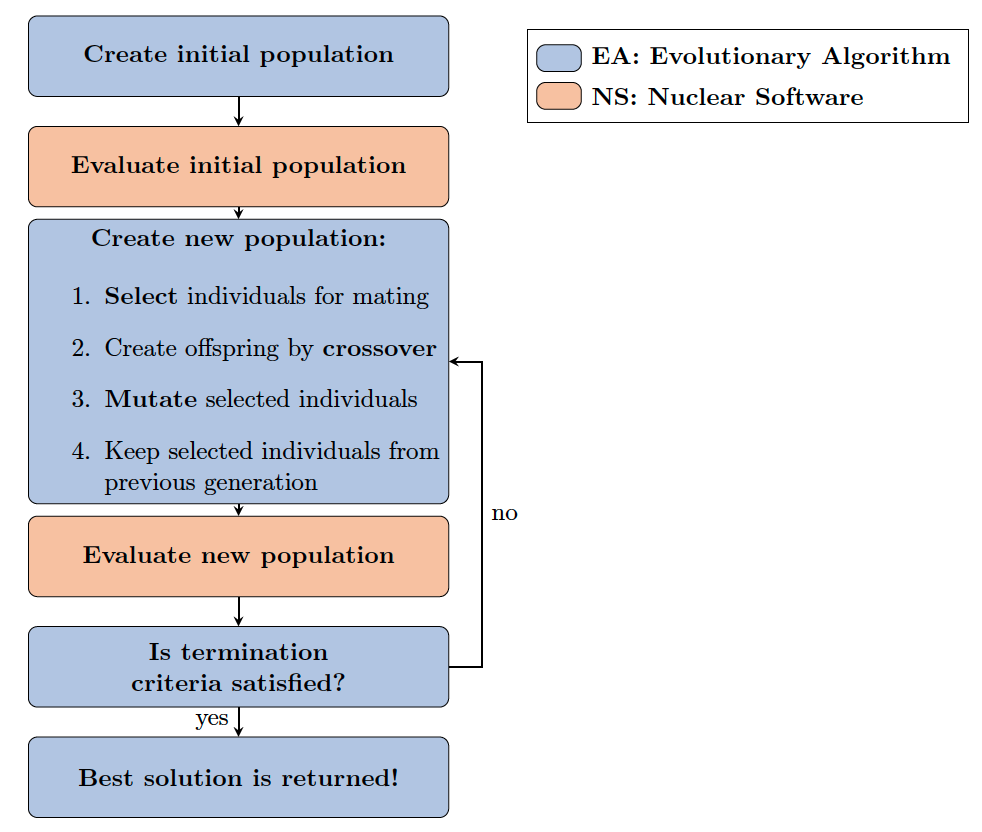
\includegraphics[width=\linewidth]{figures/rollo-flow.png} 
            \caption{Optimization tool's flow.}
        \end{figure}
    \end{minipage}
\end{frame}

\begin{frame}
    \frametitle{ROLLO: Reactor evOLutionary aLgorithm Optimizer}
    \begin{minipage}[c]{\textwidth}
        \centering
        \begin{figure}
            
\includegraphics[width=0.5\linewidth]{figures/rollo-logo.png} 
            \caption{ROLLO (Reactor evOLutionary aLgorithm Optimizer) Logo.}
        \end{figure}
    \end{minipage}
\end{frame}